\section{LDAを用いた物体のトピック分類}
物体分類を行うために(LDA

LDAではグラフィカルモデルを用いてトピック推定を行う.
\begin{figure}[h!]
	\begin{center}
		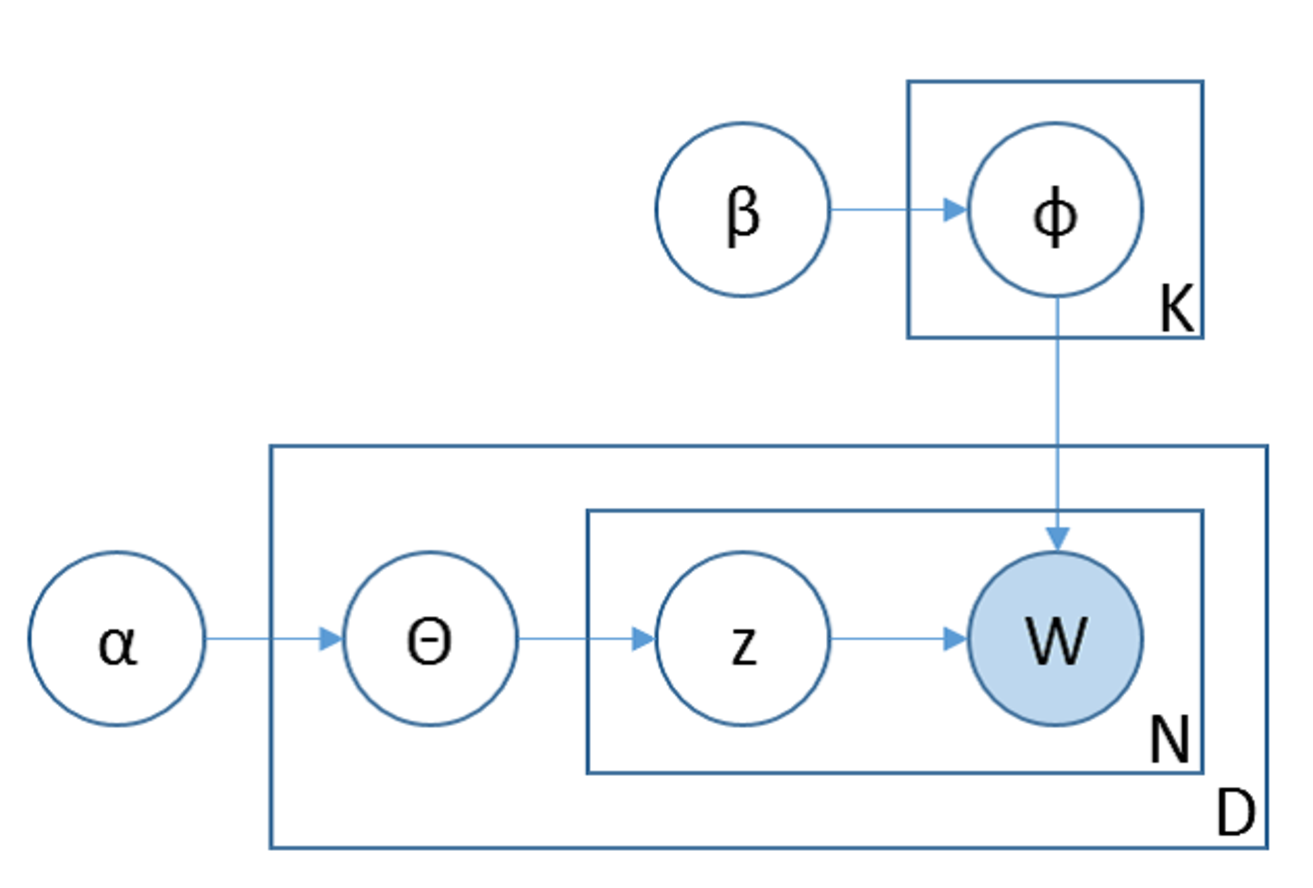
\includegraphics[width=0.30\textwidth,clip]{img/graphicalmodel.eps}
	\end{center}
	\caption{LDAにおけるグラフィカルモデル}
	\label{fig:graphical_model}
\end{figure} 
\par
%グラフィカルモデルにおける単語は入力画像をBag of Feature(BoF)によって表現する.
グラフィカルモデルにおける1ドキュメントは1画像に該当し, 
1画像の中に現れる局所特徴をBoFで表現したものが単語に該当する.
具体的には, 128次元のSIFT\cite{}を用いて変換した後, 
K平均法\cite{kmeans}を用いてベクトル量子化し, K個のクラスに分けたヒストグラムを用いる.
\par


